% ВАЖНО
% Не меняйте ничего в этом файле. А если меняете, то делайте это в этом проекте:
% https://github.com/kib-courses/latex_templates
% Для пользовательских настроек есть файл ./header/user.tex
\documentclass{beamer}
\usetheme{metropolis} 
\usecolortheme{rose}

\hypersetup{unicode=true}
\usepackage{tikz}

\usepackage{xcolor}
\usepackage[utf8]{inputenc}
\usepackage{hyphenat}
\usepackage[russian,english]{babel}          % Use metropolis theme
\usepackage{wrapfig}

\usepackage[normalem]{ulem}  % для зачекивания текста

\usepackage{caption}
\captionsetup[figure]{name=Рисунок }
\newcommand{\рис}[1]{рис.\ref{#1}}
\newcommand{\Рис}[1]{Рис.\ref{#1}}


\captionsetup[table]{name=Таблица~№}
\newcommand{\таблицa}[1]{таблица~№\ref{#1}} % именительный падеж
\newcommand{\таблицы}[1]{таблицы~№\ref{#1}} % родительный падеж
\newcommand{\таблице}[1]{таблице~№\ref{#1}} % дательный и предложный падеж
\newcommand{\таблицу}[1]{таблицу~№\ref{#1}} % винительный падеж
\newcommand{\таблицей}[1]{таблицей~№\ref{#1}} % творительный падеж 
\newcommand{\Таблицa}[1]{Таблица~№\ref{#1}} % именительный падеж
\newcommand{\Таблицы}[1]{Таблицы~№\ref{#1}} % родительный падеж
\newcommand{\Таблице}[1]{Таблице~№\ref{#1}} % дательный и предложный падеж
\newcommand{\Таблицу}[1]{Таблицу~№\ref{#1}} % винительный падеж
\newcommand{\Таблицей}[1]{Таблицей~№\ref{#1}} % творительный падеж 

\setbeamertemplate{footline}[frame number] % указывает на каждой странице общее количество страниц

% Указывайте все новые термины в \termdef команде. А уже известные ранее или из других курсов в \term
\newcommand{\termdef}[1]{\textbf{\textit{#1}}}
\newcommand{\term}{\textit}

% Диалог с аудиторией.
\newcommand{\auditorium}[1]{\textcolor{red}{\textbf{#1}}}

\let\OLDhref\href
\renewcommand{\href}[2]{\textcolor{blue}{\OLDhref{#1}{#2}}}

% \setbeameroption{show notes}
% \usepackage{listings}             % Include the listings-package
% \usepackage{minted}

\usepackage{CJKutf8}

\title{Лекция 3. RSA Risk Engine, RSA Rules Engine}
% \date{\today}
\date{8 октября 2019}
\author{Павел Владимирович Слипенчук}
\institute{Москва, МГТУ им.Бауманка,\\ каф.ИУ-8, КИБ}
% \titlegraphic{\includegraphics[width=2cm]{logo_ur.jpg}}
\titlegraphic{\small \href{https://github.com/kib-courses/dsis}{Data Science для решения задач информационной безопасности}}

\begin{document}
  \maketitle
    
\begin{frame}{План лекции}
    \begin{enumerate}
		\item \nameref{section:feedback}
		\item \nameref{section:rsa_feedback}
	\end{enumerate}
\end{frame}

\section{Обратная связь}\label{section:feedback}

\begin{frame}{Историческая заметка}
	\begin{columns}
		\begin{column}{0.5\textwidth}
			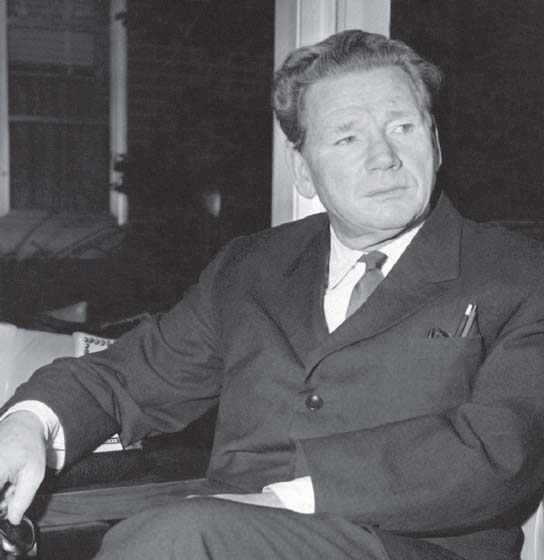
\includegraphics[width=5cm]{../pic/anohin.jpg}
		\end{column}
		\begin{column}{0.6\textwidth}
			\begin{enumerate}
				\item В 1935 году советский физиолог
				Пётр Кузьмич Анохин формулирует понятие обратной связи.
				\item Термин «перекочевал» в Кибернетику (1948) Н.Винера
				\item В настоящее время термин «обратная связь» используется в медицине, в технике, в акустике, в биологии, в социальных науках.
			\end{enumerate}
		\end{column}
	\end{columns}
\end{frame}

\begin{frame}{Обратная связь в DS}
	\termdef{Обратная связь (feedback) I}  --
	это любая информация, используемая для оценки качества ЭС
	и/или для получения новой \term{обучающей выборки} (или выборки \term{обучения с подкреплением})
	
	\termdef{Обратная связь (feedback) II} -- это процесс, система, 
	программный модуль, реализующий обратную связь I
\end{frame}

\begin{frame}{Обучение с подкреплением, reinforcement learning (Дообучение, Refitting)\footnote{слайд из лекции №2}}
	\small
	Есть первоначальная обучающая выборка: 
	\begin{equation*}
		U_{fit} = \left\{ y \mapsto \bold x  \right\}
	\end{equation*}
	Первоначальное обучение:
	\begin{equation*}
		score_1 := fit (U_{fit}) 
	\end{equation*} 
	В дальнейшем при получении нового множества $\hat U_{fit}$ (возможно состоящее из одного элемента)
	мы дообучаем систему:
	\begin{equation}
		score_{i+1} := refit (\hat U_{fit}, score_{i}) 
	\end{equation} 
	Таким образом функция $score_i$ заменяется на новую функцию $score_{i+1}$.
\end{frame}

\begin{frame}{Итеративное обучение}
	\small
	Есть первоначальная обучающая выборка: 
	\begin{equation*}
	\hat U_1 = U_{fit} = \left\{ y \mapsto \bold x  \right\}
	\end{equation*}
	Первоначальное обучение:
	\begin{equation*}
	score_1 :=   fit (\hat U_{1}) = fit (U_{fit}) 
	\end{equation*} 
	В дальнейшем при получении нового множества $\hat U_{i}$ (возможно состоящее из одного элемента)
	мы повторно обучаем систему:
	\begin{equation}
	score_{i+1} := fit ( U_{fit} \cup \hat U_2 \cup ... \cup  \hat U_{i}) 
	\end{equation} 
	Таким образом функция $score_i$ заменяется на новую функцию $score_{i+1}$.
\end{frame}

\begin{frame}
	\auditorium{Верно ли утверждение что итеративное обучение позволяет для любого алгоритма
	осуществить обучение с подкреплением?}
\end{frame}

\begin{frame}{Стабильность. <<Цепочка>>}\label{frame:chain_score}
	Есть итеративная система обучения и имеем скоринги:
	\begin{equation*}
	score_{i-n} := fit ( \hat U_{1} \cup \hat U_2 \cup ... \cup  \hat U_{i-n} \cup ... \cup \hat U_{i-1} \cup \hat U_{i}) 
	\end{equation*}
	\begin{equation*}
	...
	\end{equation*}
	\begin{equation*}
	score_{i-1} := fit ( \hat U_{1} \cup \hat U_2 \cup ... \cup  \hat U_{i-1} \cup \hat U_{i}) 
	\end{equation*}
	\begin{equation*}
	score_{i} := fit ( \hat U_{1} \cup \hat U_2 \cup ... \cup  \hat U_{i}) 
	\end{equation*}
	
	Тогда задав веса $w_j > 0$ можно сделать простой ансамбль вида:
	\begin{equation*}
	\bold {score_{i}}(\bold x) = \frac{w_1 \cdot score_{i-n}(\bold x) + ... + w_n \cdot score_{i}(\bold x)}{\sum_{j=1}^{n} w_j} 
	\end{equation*}
	
	Например:
	\begin{equation*}
	\bold {score_{i}}(\bold x) = 
		0.2 \cdot score_{i-2}(\bold x) 
		+ 0.3 \cdot score_{i-1}(\bold x) 
		+ 0.5 \cdot score_{i}(\bold x) 
	\end{equation*}
\end{frame}


\begin{frame}
	Возвращаемся к обратной связи
	\Large
	\begin{center}
		\auditorium{Зачем нужна обратная связь в DS?}
	\end{center}
\end{frame}

\begin{frame}
	Feedback позволяет:
	\begin{enumerate}
		\item Изменить $score$ на основании предыдущих \term{откликов}
		и размеченных данных. Например при каждой сработке 
		можно с вероятностью $p$ проводить расследование и дообучать систему.
		\item генетические алгоритмы: изменение параметров
		\item позволяет выявлять аномалии\footnote{<<аномалитика>> :) },
		корректировать мат.модель, выбирать из ML моделей лучшую.
	\end{enumerate}
\end{frame}


\section{RSA. Обратная связь}\label{section:rsa_feedback}

\begin{frame}{Общая схема} 
	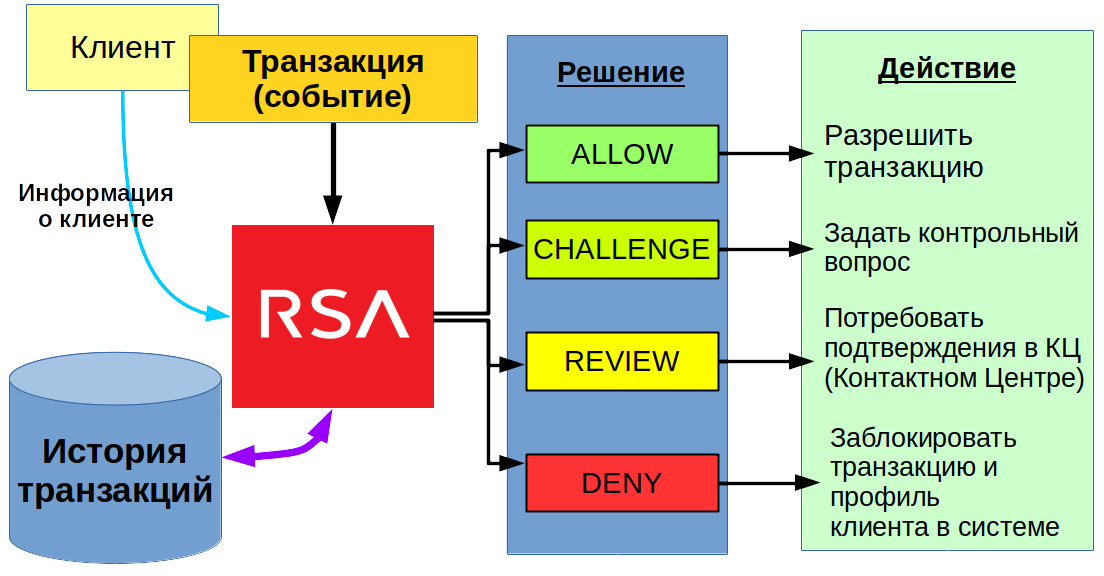
\includegraphics[width=11.5cm]{../pic/expert_system_rsa.png}
	% 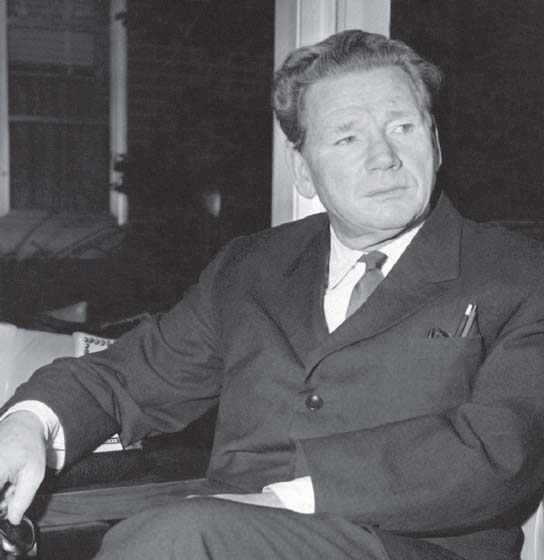
\includegraphics[width=5cm]{../pic/anohin.jpg}	
\end{frame}

\begin{frame}{Последовательность}
	% TODO заполнить последовательность действий
	\begin{enumerate}
		\item Выбираются данные за $T=90$ дней.
		% \item Выбираются <<фиксированные>> данные.
		\item Строится 
	\end{enumerate}

\end{frame}

\begin{frame}{Обратная связь. Сработки системы}\label{frame:rsa_feedback}
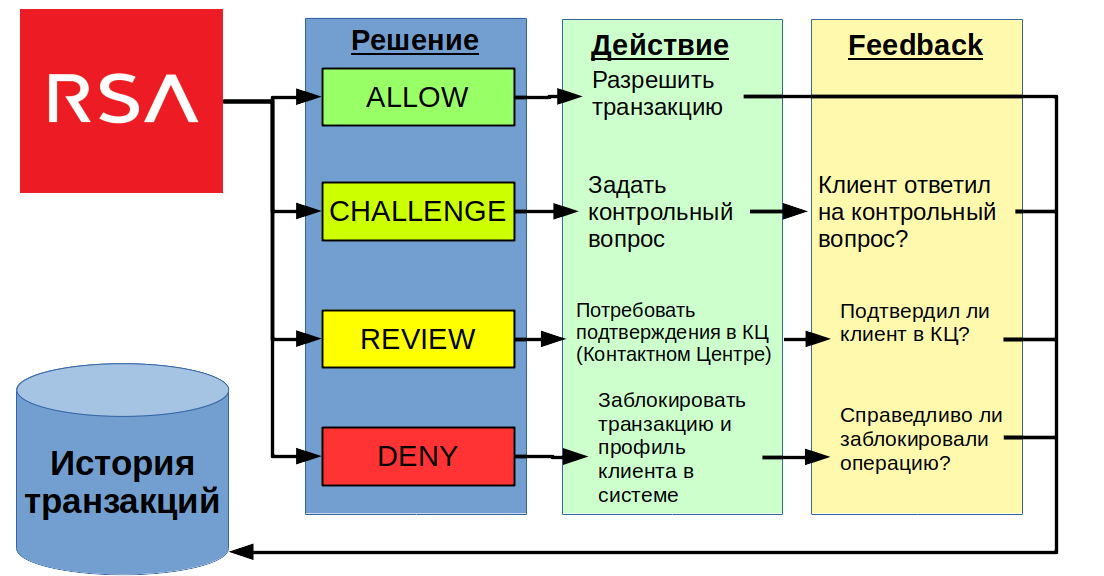
\includegraphics[width=11.5cm]{../pic/expert_system_rsa_feedback.png}
\end{frame}


\begin{frame}{Обратная связь. Жалобы}
	Если у клиента украли деньги и он это заметил, последовательность следующая:
	\begin{enumerate}
		\item клиент пишет жалобу/звонит/иным способом сообщает это
		\item специальный человек проверяет корректность жалобы. 
		Если она корректна, то данные помещаются как F.
	\end{enumerate}
	
	Контактный центр принимает звонки при всех \textbf{REVIEW} операциях.
	\auditorium{Если клиент не позвонил, какие выводы?}
	
	При \textbf{DENY} операциях проводятся специальные расследования с помощью 
	особого подразделения внутри самого банка.
\end{frame}

\begin{frame}{CUSTOM\_MARK}\label{frame:custom_mark}
	Маркировка проходит вручную.
	\begin{itemize}
		\item СUSTOM\_MARK=U (Uknoun) – неизвестная транзакция
		\item СUSTOM\_MARK=G (Genuine\footnote{RSA олдскульная система. Вместо флага L(legitim) в ней используется флаг G}) – подлинная
		\item СUSTOM\_MARK=F (Fraud) – фродовая
		\item СUSTOM\_MARK=S (Suspicious) – скорее всего фродовая
		\item СUSTOM\_MARK=A (Authentic) – скорее всего подлинная
		\item CUSTOM\_MARK=Null – не промаркировано.
	\end{itemize}
\end{frame}


\begin{frame}{Определение класса}
	По  СUSTOM\_MARK определяется класс транзакции:
	\begin{itemize}
		\item 0 -- легитимная
		\item 1 -- мошенническая
		\item x -- не используется
	\end{itemize}
	
	\begin{tabular}{|l|l|l|}
		\hline
		СUSTOM\_MARK & класс & Примечание \\ \hline
		U & x & \\ \hline
		G & 0 & \small помечаются транзакции всей сессии\\ \hline
		F & 1 & \small помечаются транзакции всей сессии\\ \hline
		S & 1 & \\ \hline
		A & 0 & \\ \hline
		Null & 0 или x & \footnotesize Спустя много дней считается легитимной\\ \hline
	\end{tabular}
\end{frame}

\begin{frame}{$AI^2$}
	Статья \textcolor{blue}{\href{https://yadi.sk/i/dJ-SrV4y3JFSPV}{<<$AI^2$: Training a big data machine to defined>>}} Kalyan Veeramachaneni, Ignacio Arnaldo и др.
	
	%\hspace{-36pt}
		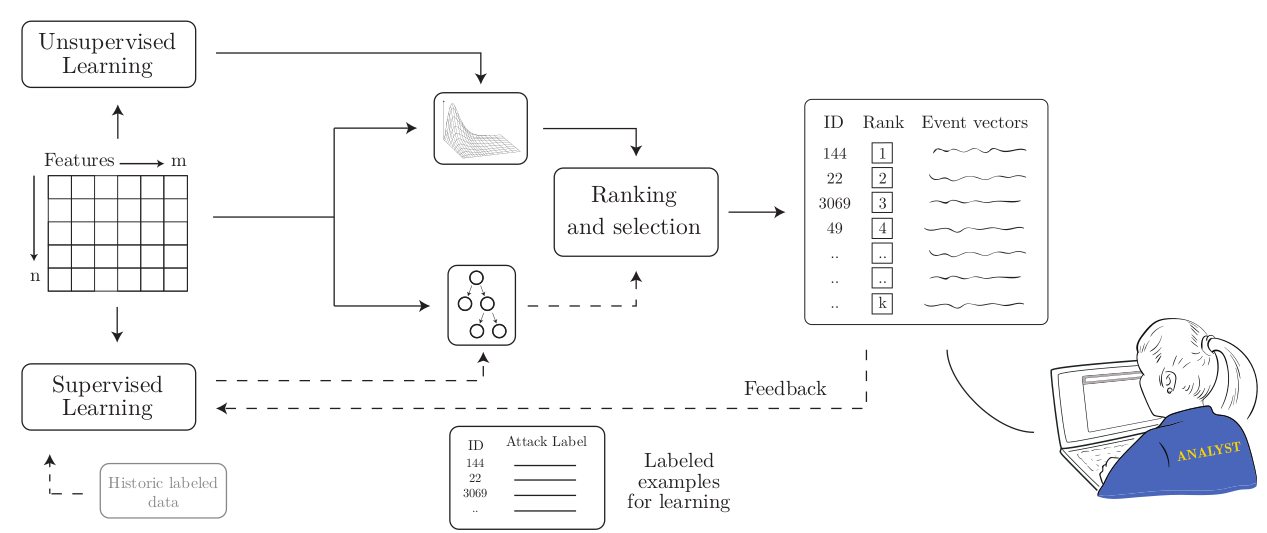
\includegraphics[width=11.5cm]{../pic/ai2_first.png}	
\end{frame}


\begin{frame}{$AI^2$}
	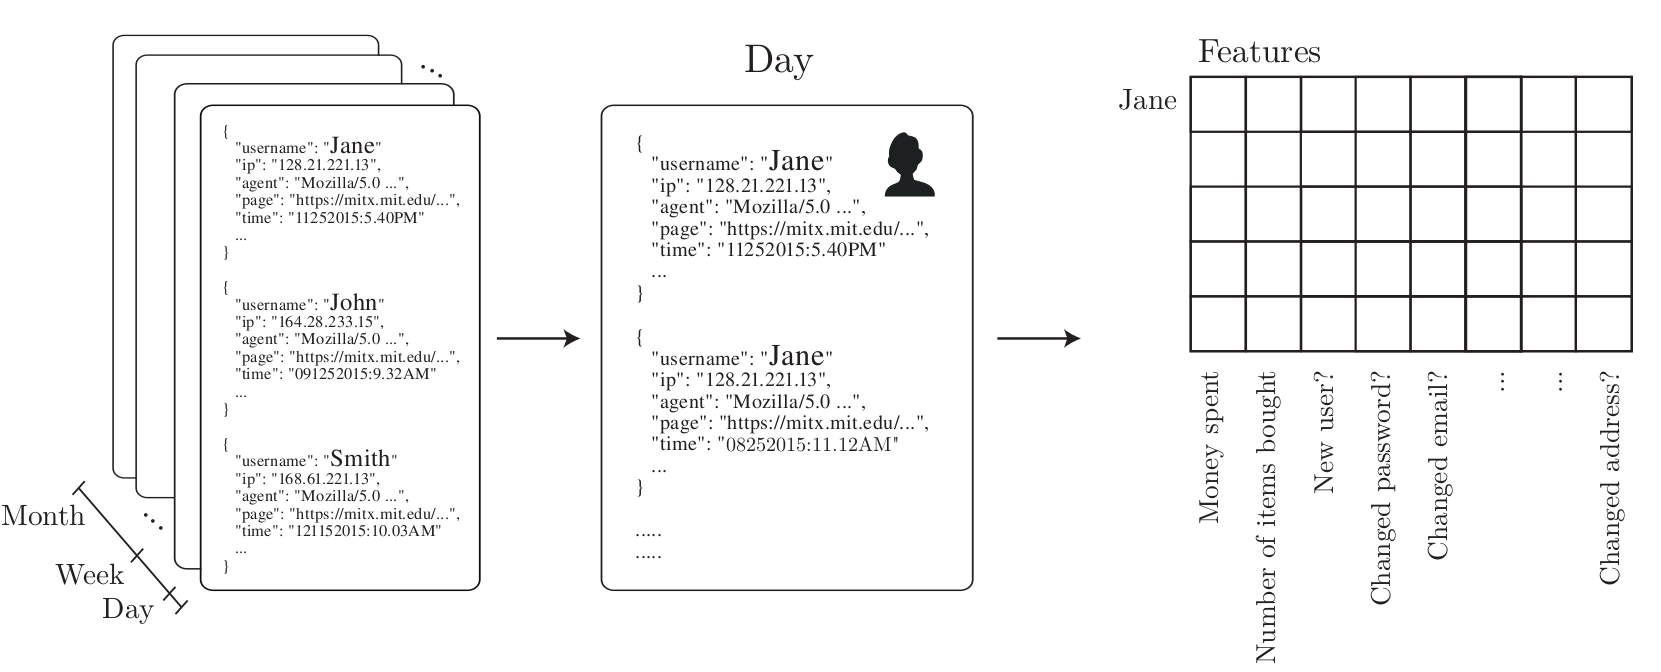
\includegraphics[width=11.5cm]{../pic/ai2_second.png}
\end{frame}

\section{RSA Rules Engine}

\begin{frame}{Risk Engine \& Rules Engine}
	\begin{itemize}
		\item \termdef{Risk Engine} -- это классификатор, 
		возвращающий значения RISK\_SCORE от 0 до 1000. 
		Чем выше это значение, тем более вероятность мошенничества.
		\item \termdef{Rules Engine} -- это ЭС,
		принимающая на вход значения \term{Risk Engine}
		и другие признаки транзакции, и выдающая решения
		ALLOW, REVIEW, CHALLANGE или DENY.
	\end{itemize}
	
	Risk Engine проектируется компанией DELL, 
	Rules Engine поставляется как движок правил. 
	
	\term{Офицеры безопасности} заказчика, используя движок Rules Engine разрабатывают 
	правила фрод мониторинга.
\end{frame}

\begin{frame}
	\begin{block}{Замечание}
		Для заказчика Risk Engine -- это чёрный ящик,
		он не вмешивается в его работу. 
		Risk Engine даётся <<as is>>, 
		или для крупных заказчиков настраивается отдельно.
	\end{block}
	\small
	Маркетинговая информация: \url{https://www.emc.com/collateral/hardware/h9096-rsa-risk-engine-sb-11-2.pdf}
\end{frame}

\begin{frame}
	
\end{frame}


\section{RSA Risk Engne}

\begin{frame}
	\begin{block}{Замечание}
	Описание Risk Engne актуально на 2015 год. Возможно многие моменты изменились 
	(вряд ли, т.к. это жёстокий энтерпрайз)
	\end{block}
\end{frame}


\begin{frame}{Контрибуторы}
	Все признаки разбиваются на 
	\termdef{контрибуторы}\footnote{\termdef{Контрибутор} (контрибьютер) -- это совокупность признаков (возможно один),
	который вносит определённый вклад в скоринговую модель. См. лекцию №2}
	по 1, 2, 3 или 4 признака, но не более. 
	
	Таким образом имеем $R^1$, $R^2$, $R^3$ или $R^4$ \term{пространство признаков}.
	
	Контрибуторы $R^n$, где $n>4$ не используются.	
\end{frame}

\begin{frame}{Скользящее окно. Разбиновка.}
	\footnotesize
	Определяем окно $\Delta_i$ для каждого $x_i$ признака 
	\term{контрибутора} 
	$(x_1, .., x_n)$
	\begin{center}
		\begin{tikzpicture}[scale=1.5]
			    \tikzstyle{F}=[circle,thick,fill=red,minimum size=1mm]
    \tikzstyle{L}=[rectangle,thick,fill=blue,minimum size=1mm]
   
    % Draw axes
    \draw [<->,thick] (0,2.3) node (yaxis) [above] {$x_2$}
        |- (4,0) node (xaxis) [right] {$x_1$};
    
    \node [F]  at (2, 1) {};
    \node [F]  at (1.8, 0.8) {};
    \node [F]  at (1.5, 0.5) {};
    \node [F]  at (1.7, 1.2) {};
    \node [F]  at (1.4, 1.5) {};
    \node [F]  at (1.2, 1) {};
    \node [F]  at (0.9, 0.3) {};
    \node [F]  at (0.3, 1.1) {};
    \node [F]  at (0.7, 0.9) {};
    \node [F]  at (0.4, 0.4) {};
    
    \node [L]  at (3.2, 1.1) {};
    \node [L]  at (2.2, 0.4) {};
    \node [L]  at (2.6, 0.6) {};
    \node [L]  at (2.3, 1.2) {};
    \node [L]  at (2.5, 1.4) {};
    \node [L]  at (2.0, 1.3) {};
    \node [L]  at (1.8, 1.8) {};
    \node [L]  at (1.6, 1.9) {};
    \node [L]  at (1.0, 1.6) {};
    \node [L]  at (0.7, 1.4) {};
    \node [L]  at (0.3, 1.6) {};
    \node [L]  at (0.6, 1.9) {};
    \node [L]  at (3.2, 0.5) {};
    \node [L]  at (3.5, 0.7) {};
    \node [L]  at (2.9, 1.3) {};
    \node [L]  at (2.8, 1.9) {};
    \node [L]  at (3.1, 1.2) {};
    \node [L]  at (3.3, 2.0) {};
    \node [L]  at (3.5, 1.1) {};
    
    
    % Выброс
    \node [F]  at (3.2, 1.6) {};
    
    % \coordinate (c) at (2, 1);
    % \fill[red] (c) circle (2pt);

    % \coordinate (c) at (1, 1);
    % \fill[red] (c) circle (2pt);

\tikzstyle{outlier}=[circle,thick,draw=black,thick, dotted,minimum size=8mm]

\draw [thick, dotted] (0.5,0) -- (0.5,2.5);
\draw [thick, dotted] (1,0) -- (1,2.5);
\draw [thick, dotted] (1.5,0) -- (1.5,2.5);

\draw [thick, loosely dotted] (2-0.015,0) -- (2-0.015,2.5);
\draw [thick, loosely dotted] (2+0.015,0) -- (2+0.015,2.5);

\draw [thick, dotted] (2.5,0) -- (2.5,2.5);

\draw [thick, loosely dotted] (3-0.015,0) -- (3-0.015,2.5);
\draw [thick, loosely dotted] (3+0.015,0) -- (3+0.015,2.5);

\draw [thick, dotted] (3.5,0) -- (3.5,2.5);


\node at (0.0,-0.2) {$a_1$};
\node at (0.5,-0.2) {$a_2$};
\node at (1.0,-0.2) {$a_3$};
\node at (1.5,-0.2) {$a_4$};
\node [outlier] at (2.0,-0.2) {$a_5$};
\node at (2.5,-0.2) {$a_6$};
\node [outlier] at (3.0,-0.2) {$a_7$};
\node at (3.5,-0.2) {$a_8$};


		\end{tikzpicture}
	\end{center}
	Определяем оптимальные бины (c помощью Индекса Джини).
	Они определяются либо в рамках отрасли (все банки), либо в рамках заказчика.
	Это -- экспертное решение DS-специалиста в рамках каждого \term{контрибутера}.
\end{frame}

\begin{frame}
	\Large
	\auditorium{Какова сложность алгоритма для $R^n$? Почему в RSA не используют контрибутеры сложности более чем 4?}
\end{frame}

\begin{frame}{Категория}
	\footnotesize
	Процедура разбиновки осуществляется либо единожды, либо при каждом повторном обучении,
	в зависимости от настроек, вручную заданные экспертом.
	
	\termdef{Категория} -- это функция скоринга контрибьютера в диапазоне $[- C_{MAX}, + C_{MAX}]$. 
	Эта величина рассчитывается в каждом бине ($bin$) через \term{Индексы Джини}:
	\begin{equation}\label{eq:category}
	C(bin) \stackrel{def}{=} log_{coef} \frac{q \cdot \Delta_1 (bin)}{\Delta_0 (bin)}
	\end{equation}
	
	Где коэффициент $coef$ задаётся экспертом вручную.
	
	Величина $q$ -- это величина, показывающая во сколько раз \textbf{во всех бинах} данных легитимных транзакций
	 больше данных мошеннических транзакций:
	\begin{equation}
	q \stackrel{def}{=} \frac{\sum_{\forall bin} \Delta_0(bin)}{\sum_{\forall bin} \Delta_1(bin)}
	\end{equation}
\end{frame}

\begin{frame}{Категория}
	\small
	Физический смысл категории в том, что если $C(bin)=0$, то данный бин не репрезентативный.
	
	Если $C(a)>0$, то $a$ скорее более мошеннический бин, чем легитимный.
	
	Если $C(b)<0$, то $b$ скорее более легитимный бин, чем мошеннический.
	
	Формула \eqref{eq:category} дополняется следующими условиями:
	\begin{enumerate}
		\item Если данных в бине мало, то $C(bin) := 0$.
		\item Если $\Delta_0 (bin) = 0$, то $C(bin) := C_{MAX} $,
		\item Если $\Delta_1 (bin) = 0$, то $C(bin) := -C_{MAX} $
		\item Если значение выходит за рамки $[-C_{MAX}, + C_{MAX}]$
		то присваивается минимально возможное / максимально возможное  значение: $-C_{MAX}$, $C_{MAX}$.
	\end{enumerate}
\end{frame}

\begin{frame}{Проблема <<скачков>> у функции логарифма}
	Так как у функции логарифма есть скачки возле нуля, то вводят \term{монотонно не убывающую} функцию $F$. Переопределим рассчёт категории:
	\begin{equation}
	C(bin) \stackrel{def}{=} F \left( log_{coef} \frac{q \cdot \Delta_1 (bin)}{\Delta_0 (bin)} \right)
	\end{equation}
	
	Что из себя представляет функция $F$ является <<коммерческой тайной RSA>>, 
	но во-первых можно догадатся, во-вторых можно проверить свою догадку, имея доступ к СУБД.
	
	\auditorium{Ваши предположения?}
\end{frame}

\begin{frame}{Группа}
	\termdef{Группа} -- это 
	\term{ансамбль}
	\term{категорий}
	вида:
	\begin{equation}
	
	\end{equation}
\end{frame}


\begin{frame}{Термины RSA}\label{frame:rsa_risk_engine_terms}
	\auditorium{Вопрос к залу. Who is who?}
	\begin{enumerate}
		\item Разбиновка 
		\item Категория. $R^1$, $R^2$, $R^3$, $R^4$ категории
	
	\end{enumerate}
\end{frame}


  
\section{Вопросы для самопроверки}

\begin{frame}
	Прочитайте, что такое <<генетические алгоритмы>>(genetic algorithm).
	В чём роль обратной связи в них?
	
	Предложите структуру гена генетического алгоритма, создающий стратегии игры в крестики нолики. 
	
	Для желающих: реализуйте его (вместо какой-нибудь лабораторной). 
	<<стравите>> разные гены друг с другом и путём <<эволюции>>
	получите самый сильный алгоритм.
	
	Стал ли полученный алгоритм оптимальным? Сыграйте несколько партий. Сколько раз выиграли, 
	сколько проиграли, сколько раз сыграли вничью?
	
\end{frame}

\begin{frame}{Обратная связь и итеративное обучение}
	\begin{enumerate}
		\item В <<цепочке>> (см. слайд №\ref{frame:chain_score}) задана функция
		$\bold score$ с коэффициентами $(0.1, 0.2, 0.7)$. Каков будет скоринг, 
		если $score_1=540$, $score_2=546$, $score_3=584$?
		\item В <<цепочке>> задана функция 	$\bold score$ 
		с коэффициентами $(0.2, 0.4, 0.8)$. Значения $score_1, score_2, score_3$
		равны $345$, $124$ и $573$. Почему $\bold {score}$ 
		будет $412$, 
		а не $577$ ?
		\item Предположим, что $score_{i+1}$ 
		сильно больше чем $score_i$. Что это значит? 
		Действительно ли система работает нестабильно? 
		Приведите контрпримеры.
		
	\end{enumerate}
\end{frame}

\begin{frame}{RSA}
	\begin{itemize}
		\item На слайде №\ref{frame:rsa_feedback} не указаны действия
		обратной связи для ALLOW операции. Т.е. не производится никаких работ. 
		Почему?
		\item На слайде №\ref{frame:rsa_feedback} не указан процесс получения 
		по жалобам клиентов. По каким решениям ФМ системы возможны жалобы? 
		Приведите пример жалоб для ALLOW систем. 
		\item Почему если произошла операция DENY на правило "перевыпуск СИМ карт", 
		сотрудники коллцентра не могут разблокировать профиль позвонившим
		недовольным клиентам банка? Почему необходима либо более сложная аутентификация, чем 
		телефонный звонок?
	\end{itemize}
\end{frame}

\begin{frame}{RSA}
\begin{itemize}
	\item Почему большинство транзакций имеют CUSTOM\_MARK=Null ?
	(см. слайд №\ref{frame:custom_mark})
	\item Почему все непромаркированные операции (CUSTOM\_MARK=Null) спустя 10 и более дней считаются 
	легитимными в обучающей выборке?
\end{itemize}
\end{frame}

\begin{frame}{Risk Engine}
	\begin{enumerate}
		\item 	Ответьте на вопросы о терминологии \mbox{Risk Engine}
		со слайда №\ref{frame:rsa_risk_engine_terms}
		\item Посмотрите на формулу \eqref{eq:category}. Зачем нужно брать логарифм?
		Почему бы просто не поделить (умножить) на $coef$?  
		\item Что будет, если не использовать коэфициент $q$ в формуле \eqref{eq:category} ?
		\item Если бы $q$ задавали бы формулой:
		\begin{equation*}
		q \stackrel{def}{=} \frac{\sum_{\forall bin} \Delta_1(bin)}{\sum_{\forall bin} \Delta_0(bin)}
		\end{equation*}
		то как бы изменилась формула \eqref{eq:category}?
	\end{enumerate}
\end{frame}



\end{document}